\documentclass[rgb]{beamer}

\usepackage[english]{babel}
\usepackage[utf8]{inputenc}
\usepackage{xcolor}
\usepackage{listings}
\usepackage{adjustbox}
\usepackage{amsmath}
\usepackage{multirow}
\usepackage[linewidth=1pt]{mdframed}

% Graphics
\usepackage{graphicx}

\usepackage{tikz}
\usetikzlibrary{calc,shapes.multipart,chains,arrows}

% Font
\usepackage{paratype}
\setbeamerfont{frametitle}{family=\bf}

% Beamer theme settings
\usecolortheme{seagull}
\setbeamertemplate{itemize item}{\raisebox{0.8mm}{\rule{1.8mm}{1.2mm}}}
\usenavigationsymbolstemplate{} % no navigation buttons

\usepackage{listings}

% Define Language
\lstdefinelanguage{fsharp}
{
  % list of keywords
  morekeywords={
    and,
    do,
    else,
    exception,
    for,
    fun,
    function,
    if,
    in,
    let,
    match,
    module,
    mutable,
    open,
    of,
    rec,
    then,
    try,
    type,
    unsafe,
    use,
    val,
    when,
    while,
    with,
  },
  sensitive=true, % keywords are not case-sensitive
  morecomment=[l]{//}, % l is for line comment
%  otherkeywords={>,<,=,<=,>=,!,*,/,-,+,|,&,||,&&,==,=>},
  morestring=[b]" % defines that strings are enclosed in double quotes
}

% Define Colors
\usepackage{color}
\definecolor{eclipseBlue}{RGB}{42,0.0,255}
\definecolor{eclipseGreen}{RGB}{63,127,95}
\definecolor{eclipsePurple}{RGB}{127,0,85}

\newcommand{\fop}[1]{\mbox{\ttfamily\color{eclipseBlue}#1}}
\newcommand{\fw}[1]{\mbox{\ttfamily\bfseries\color{eclipsePurple}#1}}

% Set Language
\lstset{
  language={fsharp},
  basicstyle=\ttfamily, % Global Code Style
  captionpos=b, % Position of the Caption (t for top, b for bottom)
  extendedchars=true, % Allows 256 instead of 128 ASCII characters
  tabsize=2, % number of spaces indented when discovering a tab
  columns=fixed, % make all characters equal width
  keepspaces=true, % does not ignore spaces to fit width, convert tabs to spaces
  showstringspaces=false, % lets spaces in strings appear as real spaces
  breaklines=true, % wrap lines if they don't fit
  frame=trbl, % draw a frame at the top, right, left and bottom of the listing
  frameround=tttt, % make the frame round at all four corners
  framesep=4pt, % quarter circle size of the round corners
  numbers=left, % show line numbers at the left
  numberstyle=\small\ttfamily, % style of the line numbers
  commentstyle=\slshape\bfseries\color{eclipseGreen}, % style of comments
  keywordstyle=\bfseries\color{eclipsePurple}, % style of keywords
  stringstyle=\color{eclipseBlue}, % style of strings
  emph=[1] {
    false,
    true,
    Set,
    Map,
    List,
    ImgUtil,
    Pegs,
    String,
    Array,
    Array2D
  },
  emphstyle=[1]{\color{eclipseBlue}},
  moredelim=**[is][\color{red}]{@@}{@@}
}

\newcommand{\theyear}{2020}
\newcommand{\sem}[1]{[\![#1]\!]}
\newcommand{\seme}[1]{\sem{#1}\varepsilon}
\newcommand{\semzero}[1]{\sem{#1}_0}

\newcommand{\emptymap}{\{\}}
\newcommand{\fracc}[2]{\begin{eqnarray} \frac{\begin{array}{c} #1
    \end{array}}{\begin{array}{c} #2 \end{array}} \end{eqnarray}}
\newcommand{\sembox}[1]{\hfill \normalfont \mbox{\fbox{\(#1\)}}}
\newcommand{\sempart}[2]{\subsubsection*{\rm\em #1 \sembox{#2}}}
\newcommand{\axiom}[1]{\begin{eqnarray} \begin{array}{c} #1 \end{array} \end{eqnarray}}
\newcommand{\fraccn}[2]{\refstepcounter{equation}\mbox{$\frac{\begin{array}{c} #1 \end{array}}{\begin{array}{c} #2 \end{array}}$}~(\arabic{equation})}
\newcommand{\fraccc}[2]{\mbox{$\frac{\begin{array}{c} #1 \end{array}}{\begin{array}{c} #2 \end{array}}$}}
\newcommand{\onepart}[1]{\noindent\hfill#1\hfill~\vspace{2mm}}
\newcommand{\twopart}[2]{\noindent\hfill#1\hfill#2\hfill~\vspace{2mm}}
\newcommand{\threepart}[3]{\noindent\hfill#1\hfill#2\hfill#3\hfill~\vspace{2mm}}
%\newcommand{\axiomm}[1]{\refstepcounter{equation}\mbox{$\begin{array}{c} #1 \end{array}$}~(\arabic{equation})}
\newcommand{\axiomm}[1]{$\begin{array}{c} #1 \end{array}$}
%\newcommand{\ar}[1]{\stackrel{#1}{\longrightarrow}}
\newcommand{\vd}{\vdash}
\newcommand{\Ran}{{\rm Ran}}
\newcommand{\Dom}{{\rm Dom}}
\newcommand{\kw}[1]{\texttt{#1}}
\newcommand{\id}[1]{\mbox{\it{#1}}}
\newcommand{\rarr}{\rightarrow}
\newcommand{\eval}{\rarr}
\newcommand{\evals}{\leadsto}
\newcommand{\larr}{\leftarrow}

\newcommand{\head}[1]{\vspace{3mm} \textbf{\normalsize #1}}
\newcommand{\headsp}[1]{\head{#1}\vspace{1ex}}
\newcommand{\size}{\ensuremath{\mathrm{size}}}
\renewcommand{\log}{\ensuremath{\mathrm{log}}}

\newcommand{\setallthemecolors}[1]{%
\setbeamercolor*{palette primary}{use=structure,fg=white,bg=#1}%
\setbeamercolor*{palette secondary}{use=structure,fg=white,bg=#1}%
\setbeamercolor*{palette tertiary}{use=structure,fg=white,bg=#1}}

\definecolor{black}{RGB}{0,0,0}
\definecolor{maroon}{RGB}{128,0,0}
\definecolor{olive}{RGB}{128,128,0}
\definecolor{green}{RGB}{0,128,0}
\definecolor{purple}{RGB}{128,0,128}
\definecolor{teal}{RGB}{0,128,128}
\definecolor{darkteal}{RGB}{0,92,92}
\definecolor{navy}{RGB}{0,0,128}
\definecolor{gray}{RGB}{128,128,128}
\definecolor{darkgray}{RGB}{60,60,60}
\definecolor{darkred}{RGB}{139,0,0}

%palette

% #173F5F (dark blue)
\definecolor{darkblue}{RGB}{23,63,95}
% #20639B (blue)
\definecolor{blue}{RGB}{32,99,155}
% #3CAEA3 (green)
\definecolor{magenta}{RGB}{60,174,163}
% #F6D55C (yellow)
\definecolor{yellow}{RGB}{246,213,92}
% #ED553B (red)
\definecolor{red}{RGB}{237,85,59}


\usecolortheme{whale}
\useoutertheme{infolines}
\useinnertheme{rectangles}

\newcommand{\popsettitle}[2]{%
\setallthemecolors{#1}%
\newcommand{\popemne}{#2}%
\title{Programmering og Problemløsning}%
\subtitle{#2}%
\author{Martin Elsman}%
\date{}%
\institute[DIKU]{Datalogisk Institut, Københavns Universitet (DIKU)}}

\newcommand{\popmaketitleframe}{%
  \frame{\titlepage%
   \vspace{-15mm}%
   \par\noindent\rule{\textwidth}{0.4pt}%

   \vspace{4mm}%
   \tableofcontents%
   \vspace{-4mm}%
   \par\noindent\rule{\textwidth}{0.4pt}%
  }%
  \section*{\popemne}%
}


\popsettitle{darkteal}{Træstrukturer (Del 1)}  % see ../util.tex for colors

\begin{document}

\popmaketitleframe

%%%%%%%%%%%%%%%%%%%%%%%%%%%%%%%%%%%%%%%%%%%%%%%%
%\subsection{Introduktion}
%%%%%%%%%%%%%%%%%%%%%%%%%%%%%%%%%%%%%%%%%%%%%%%%

\subsection{Rekursive sum-typer}

\begin{frame}[fragile]
\begin{footnotesize}

  \head{Introduktion til rekursive sum-typer}
  \vspace{1ex}

  Rekursive sum-typer er sum-typer der kan have konstruktører der tager argumenter hvis type refererer til sum-typen selv!

  \vspace{1ex}

  \head{Eksempel:}

\begin{lstlisting}[numbers=none,frame=none,mathescape]
  type expr = Const of int            // Expression trees
            | Add of expr * expr
            | Mul of expr * expr
\end{lstlisting}

  \vspace{1ex}
  Med simple rekursive funktioner er beregninger på sådanne sum-typer mulig:

  \vspace{1ex}
\begin{minipage}{0.7\textwidth}
  \head{Eksempel:}
  \begin{lstlisting}[numbers=none,frame=none,mathescape]
  let rec eval (e:expr) : int =
    match e with
    | Const c -> c
    | Add (a,b) -> eval a + eval b
    | Mul (a,b) -> eval a * eval b

  let x = Add(Mul(Const 3,Const 8),Const 8)
  do printfn "eval(x)=%d" (eval x)
\end{lstlisting}
\end{minipage}\begin{minipage}{0.25\textwidth}
\vspace{-1cm}~\hspace{-1cm}
  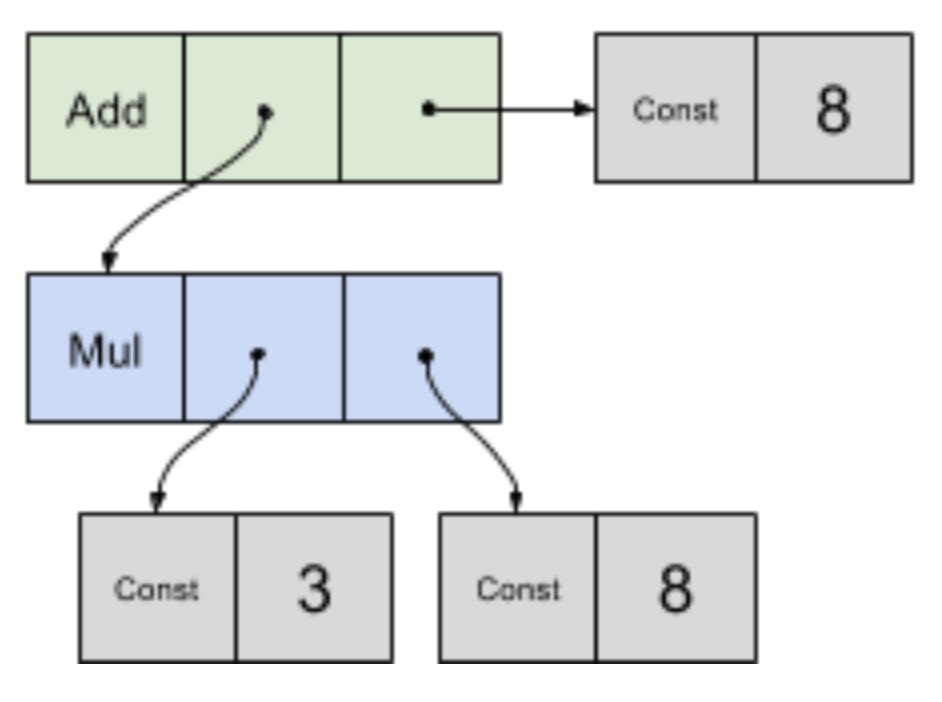
\includegraphics[width=1.4\textwidth]{../images/addmul.png}

\end{minipage}

\end{footnotesize}
\end{frame}

\begin{frame}[fragile]
\begin{footnotesize}

  \head{Rekursive Sum-typer kan være type-generiske.}
  \vspace{1ex}

  Rekursive sum-type definitioner kan (ligesom ordinære sum-typer) være \emph{generiske} således at de er
  parameteriserede over en eller flere typer.

  \vspace{1ex}

\head{En generisk træ-type er et godt eksempel:}

\begin{lstlisting}[numbers=none,frame=none,mathescape]
  type 'a tree = Leaf of 'a | Tree of 'a tree * 'a tree
\end{lstlisting}

  \vspace{1ex}
  \head{Vi kan nu skrive generisk (genbrugelig) kode:}
\begin{lstlisting}[numbers=none,frame=none,mathescape]
  let rec depth (t:'a tree) : int =
    match t with
    | Leaf _ -> 1
    | Tree (t1,t2) -> 1 + max (depth t1) (depth t2)
\end{lstlisting}

  \vspace{1ex}

  \head{Her er en funktion som kun virker på specialiserede træer:}
\begin{lstlisting}[numbers=none,frame=none,mathescape]
  let rec sum (t:int tree) : int =
    match t with
    | Leaf x -> x
    | Tree (t1,t2) -> sum t1 + sum t2
\end{lstlisting}

\end{footnotesize}
\end{frame}

\subsection{Forskellige typer træer}

\begin{frame}[fragile]
\begin{footnotesize}

  \headsp{Træer med værdier i bladene (fortsat)}

  Vi betragter fortsat træer med værdierne gemt i \textbf{bladene}:

  \vspace{1ex}

\begin{lstlisting}[numbers=none,frame=none,mathescape]
type 'a tree = Leaf of 'a | Tree of 'a tree * 'a tree
\end{lstlisting}
  \vspace{1ex}

Sådanne træer kan være anvendelige f.eks. i forbindelse med at gøre streng-sammensætning effektiv.

\headsp{Betragt følgende kode:}

\begin{lstlisting}[numbers=none,frame=none,mathescape]
  let rec loop i =
    if i < 1 then "" else loop (i-1) + string i
  in loop 50000
\end{lstlisting}

\vspace{1ex}
Problemet kan også ses i følgende kode:
\vspace{1ex}
\begin{lstlisting}[numbers=none,frame=none,mathescape]
  let problematic = "hello" + " " + "world"
\end{lstlisting}

\end{footnotesize}
\end{frame}

\begin{frame}[fragile]
\begin{footnotesize}

  \head{Vi kan i stedet opbygge et træ --- \texttt{cstest.fs}:}
  \vspace{1ex}
\begin{lstlisting}[numbers=none,frame=none,mathescape]
  let (++) x y = Tree (x,y)    // infix operator definition
  let S s = Leaf s             // simple leaf construktor
  let rec csloop i : string tree =
    if i < 1 then S"" else csloop (i-1) ++ S(string i)
  let cs = S"Numbers from 1 to 50000:\n" ++ csloop 50000
\end{lstlisting}

  \vspace{1ex}
  \head{Konstruktion af den færdige streng:}
  \vspace{1ex}
\begin{lstlisting}[numbers=none,frame=none,mathescape]
  let rec flatten (acc:'a list) (t:'a tree) : 'a list =
    match t with
    | Leaf s -> s :: acc
    | Tree (x,y) -> flatten (flatten acc y) x

  let toString (x:string tree) : string =
    String.concat "" (flatten [] x)    // 50000x speedup!
\end{lstlisting}

\end{footnotesize}
\end{frame}

\begin{frame}[fragile]
\begin{footnotesize}

  \head{Eksempel: HTML generering}
  \vspace{1ex}
\begin{lstlisting}[numbers=none,frame=none,mathescape]
module Html
type html
val S        : string -> html
val tag      : string -> html -> html
val (++)     : html -> html -> html
val toString : html -> string
\end{lstlisting}

\head{Implementation:}
  \vspace{1ex}
\begin{lstlisting}[numbers=none,frame=none,mathescape]
module Html
type html = string tree
let S s = Leaf s
let (++) x y = Tree (x,y)    // infix operator definition
let tag t e = S("<"+t+">") ++ e ++ S("</"+t+">")
let toString (x:html) : string =
  String.concat "" (flatten [] x)
\end{lstlisting}

\end{footnotesize}
\end{frame}

\begin{frame}[fragile]
\begin{footnotesize}

  \head{Eksempel: HTML generering --- brug af bibliotek}

  \vspace{1ex}
\begin{lstlisting}[numbers=none,frame=none,mathescape]
> toString(tag "h2" (S"Nice world"));;
val it : string = "<h2>Nice world</h2>"
\end{lstlisting}

  \vspace{1ex}
  \head{Mere interessant kode:}

  \vspace{1ex}

\begin{lstlisting}[numbers=none,frame=none,mathescape]
let flat (xs:html list) : html =
  List.foldBack (fun x acc -> x ++ acc) xs (S"")

let intitems (xs:int list) : html =
  let es = List.map (fun x -> tag "li" (S(string x))) xs
  tag "ul" (flat es)

let rec fib n = if n <= 2 then 1 else fib (n-1) + fib (n-2)

let doc =
  let fibs = List.map fib [1..10]
  in tag "html" (tag "body" (tag "h2" (S"Fibs") ++
                             intitems fibs))
\end{lstlisting}

\end{footnotesize}
\end{frame}

\begin{frame}[fragile]
\begin{footnotesize}

  \head{Eksempel: HTML generering --- output --- \texttt{html.fs}:}

  \vspace{1ex}
  \lstinline{toString doc} giver følgende output:
  \vspace{5mm}

\begin{minipage}{0.8\textwidth}
\begin{verbatim}
<html>
  <body>
    <h2>Fibs</h2>
    <ul><li>1</li><li>1</li><li>2</li>
        <li>3</li><li>5</li><li>8</li>
        <li>13</li><li>21</li><li>34</li>
        <li>55</li>
    </ul>
  </body>
</html>
\end{verbatim}
\end{minipage}\begin{minipage}{0.15\textwidth}
  \fbox{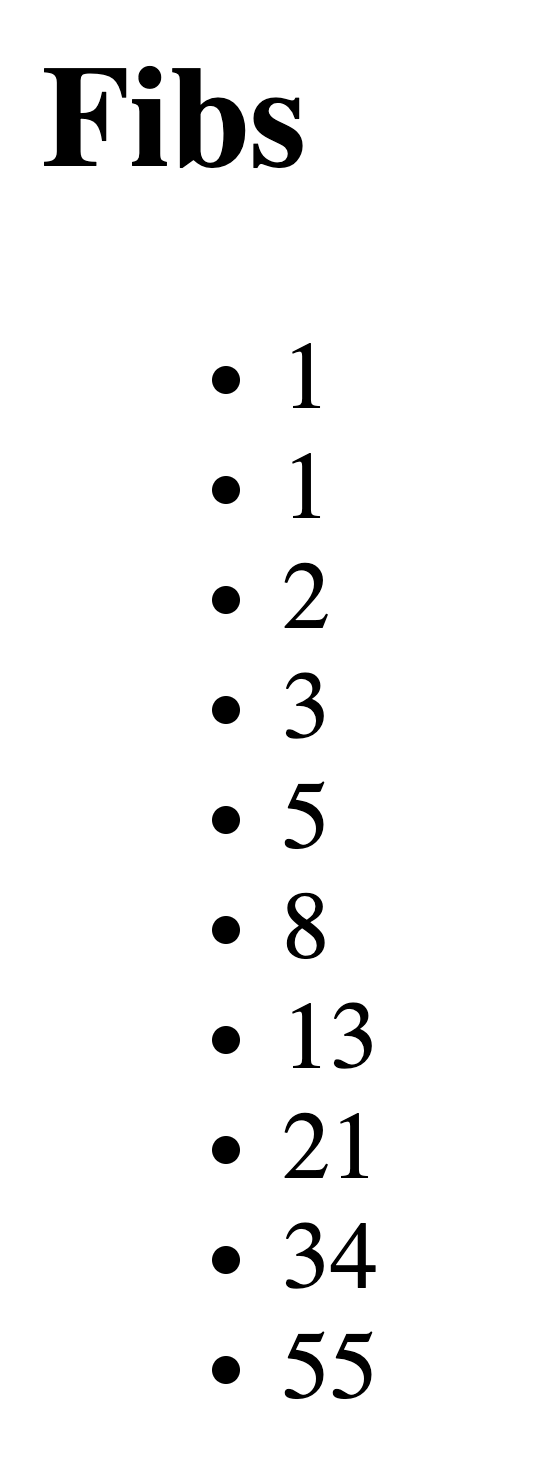
\includegraphics[width=.8\textwidth]{../images/fibweb.png}}
  \vspace{-5mm}
\end{minipage}


\vspace{1ex}

  \head{Bemærk:}
  \vspace{1ex}
  \begin{itemize}
  \item Det er let at konstruere nye interessante kombinatorer der kan bygge tabeller, etc.
  \item Vi skal senere se hvordan vi kan gemme den genererede HTML-kode i en HTML-fil.
  \item Teknikken kan også bruges i en \textbf{web-server} der serverer HTML-kode eller anden XML-formateret kode til klienter (web-browsere).
  \end{itemize}

\end{footnotesize}
\end{frame}

\begin{frame}[fragile]
\begin{footnotesize}

  \head{Træer med værdier i forgreningerne}
  \vspace{1ex}

  I følgende definition af et træ er værdierne gemt i \textbf{forgreningerne}:

  \vspace{1ex}

\begin{lstlisting}[numbers=none,frame=none,mathescape]
type 'a t = L | T of 'a t * 'a * 'a t
\end{lstlisting}
  \vspace{1ex}

Funktion til opbygning af balanceret træ:
  \vspace{1ex}
\begin{lstlisting}[numbers=none,frame=none,mathescape]
let rec build (l:'a list) : 'a t =
  match List.splitAt (List.length l/2) l with
  | ([],[]) -> L
  | (l1,x::l2) -> T(build l1,x,build l2)
  | _ -> failwith "impossible"
\end{lstlisting}

  \vspace{1ex}

  \head{Spørgsmål:}
  \vspace{1ex}
  \begin{itemize}
  \item Hvad kan et sådan balanceret træ bruges til?
  \end{itemize}

\end{footnotesize}
\end{frame}

\begin{frame}[fragile]
\begin{footnotesize}

  \head{Balancerede træer kan fint bruges til søgetræer}
  \vspace{1ex}

  \vspace{1ex}

\begin{minipage}[b]{0.7\textwidth}

  Her er en funktion til at afgøre om et element er i træet:
  \vspace{1ex}
\begin{lstlisting}[numbers=none,frame=none,mathescape]
  let rec mem (t:int t) (v:int) : bool =
    match t with
    | L -> false
    | T(left,x,right) ->
     if v < x then mem left v
     else if v > x then mem right v
     else true
\end{lstlisting}
\end{minipage}
\begin{minipage}[b]{0.25\textwidth}

  ~\hspace{-5mm}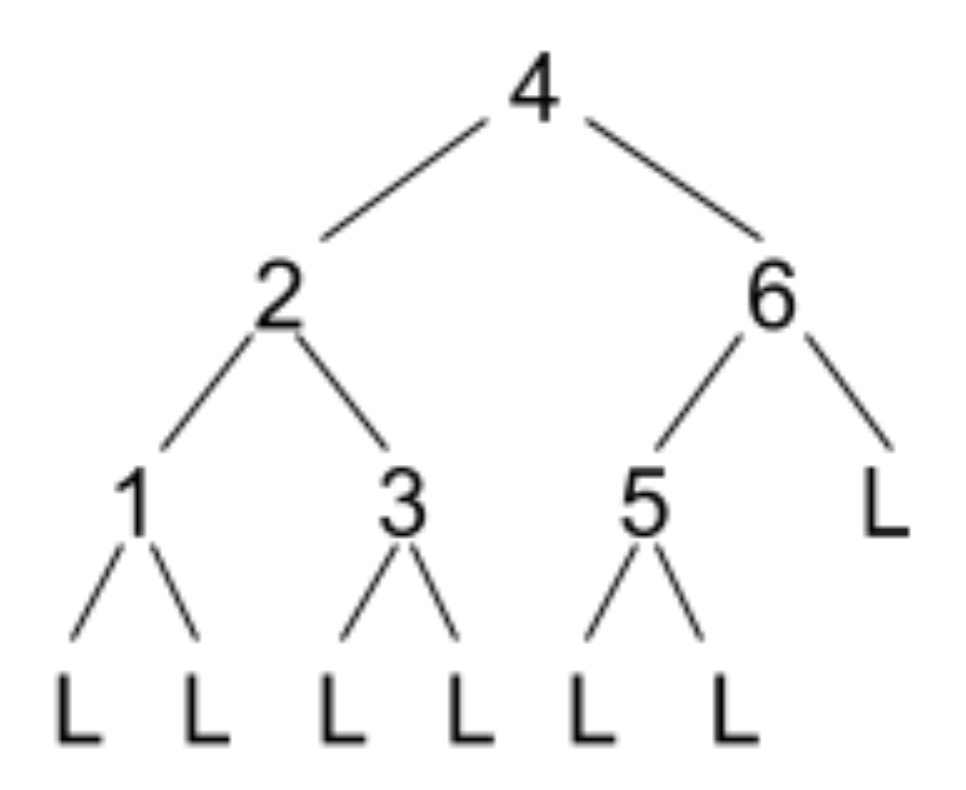
\includegraphics[width=1.2\textwidth]{../images/tree123456.png}

\end{minipage}

  \vspace{1ex}
  \head{Bemærk:}
  \vspace{1ex}
  \begin{itemize}
  \item Der skal højst benyttes $O(\log N)$ operationer til at afgøre om et element er i træet.
  \item Balancerede træer kan således fint benyttes til repræsentation af mængder.
  \item Hvilke begrænsninger har den simple sum-type vi har givet?
  \end{itemize}

\end{footnotesize}
\end{frame}

\subsection{Gennemløb af træstrukturer}

\begin{frame}[fragile]
\begin{footnotesize}

  \head{Gennemløb af træstrukturer}
  \vspace{1ex}

  Vi så i HTML-eksemplet hvordan vi kunne etablere en liste indeholdende informationen i alle bladene i et træ.

  \vspace{1ex}
  \head{Andre træ-operationer}
  \begin{itemize}
  \item map : omform data i bladene (eller knuderne)
  \item fold(Back) : akkumul\'{e}r data i bladene eller knuderne (forfra eller bagfra)

    (her er der mange muligheder, afhængigt af i hvilken rækkefølge knuder skal processeres)
  \item indsætning
  \item sletning af element
  \item (re)balancering
  \item pretty-printing
  \end{itemize}
\end{footnotesize}
\end{frame}

\subsection*{Konklusion}
\begin{frame}[fragile]
  \headsp{Konklusion}

  \vspace{3mm}
  \tableofcontents
\end{frame}

\end{document}
